\documentclass[skript.tex]{subfiles}

\begin{document}

	\begin{bem}
		Für stetige und Lebesgue-integrierbare Funktionen auf reellen Intervallen stimmen
		Riemann- und Lebesgue-Integral überein. \\
		Sei $f \in C^0 (a,b)$ Lebesgue-integrierbar auf $(a,b)$. \\
		Wir setzen
		\[
			F(x) = \lint_{(a,x]} f \md\lambda\,, \quad x \in (a,b)
		\]
		Wir behaupten $F \in C^1(a,b)$ mit $F'(x) = f(x) \; \forall x \in (a,b)$. \\ 
		In der Tat, für $\epsilon > 0$ ist
		\begin{align*}
			\frac{F(x+\epsilon)-F(x)}{\epsilon} &\darrow{\text{Lem. 43}}{=}
			\frac{1}{\epsilon} \lint_{(x,x+\epsilon]} f(\xi) \md \lambda(\xi)
			= \frac{1}{\epsilon} \lint_{(x,x+\epsilon]} (f(x)+f(\xi)-f(x)) \md \lambda(\xi)
			\\ &\darrow{\text{Lem. 43}}{=}
			\frac{1}{\epsilon}\lint_{(x,x+\epsilon]} f(x) \md \lambda(\xi)
			+ \frac{1}{\epsilon}\lint_{(x,x+\epsilon]} 
			\underbrace{(f(\xi)-f(x))}_{
				\mathrlap{
					\leq sup_{\eta\in(x,x+\epsilon]} |f(\eta)-f(x)|
				}
			}
			\md \lambda(\xi) \\
			&\darrow{\text{Lem. 45}}{\leq}
			\frac{1}{\epsilon} f(x)
			\underbrace{\lambda\big((x,x+\epsilon]\big)}_\epsilon
			+ \frac{1}{\epsilon} \lambda\big((x,x+\epsilon]\big) \sup | f(\eta)-f(x)|.
		\end{align*}
		Wir haben also
		\[
			\frac{F(x+\epsilon)-F(x)}{\epsilon}
			= f(x) + \lint_{(x,x+\epsilon]}(f(\xi)-f(x)) \md \lambda(\xi)
		\]
		mit
		\[
			\left|\lint_{(x,x+\epsilon]}(f(\xi)-f(x)) \md \lambda(\xi)\right|
			\overset{\text{L. 51}}{\leq}
			\frac{1}{\epsilon} \lint_{(x,x+\epsilon]}|f(\xi)-f(x)| \md \lambda(\xi)
			\leq \sup_{\eta\in(x,x+\epsilon]} |f(\eta)-f(x)|
			\underset{\text{Stetigk.}}{\xrightarrow{\epsilon\searrow 0}} 0.
		\]
		Für $\epsilon < 0$ argumentiere analog. \\
		Ist $f$ stetig auf einem kompakten Intervall, so ist $f$ beschränkt und messbar,
		also Lebesgue-integrierbar.\\
		
		Allgemeiner ist jede beschränkte messbare Funktion auf einem kompakten
		Intervall genau dann Riemann-integrierbar, wenn die Menge ihrer Unstetigkeitsstellen eine Lebesgue-Nullmenge ist. \\
		In diesem Fall stimmen Riemann- und Lebesgue-Integral überein. Diese Aussage gilt nicht für verallgemeinerte Intervalle.
	\end{bem}

	\begin{bsp*}
		$\int_0^\infty \frac{\sin x}{x} \md x$ existiert als Riemann-Integral
		$\lim_{R\nearrow\infty} \int_0^R \frac{\sin(x)}{x} \md x$, andererseits ist \\
		$\int_0^\infty\left|\frac{\sin x}{x}\right| \md x = \infty$, also keine
		Lebesgue-Integrierbarkeit.
	\end{bsp*}

	\section{Produktmaße}
	\begin{notat}
		Für Messräume $(X_1,\Sigma_1)$, $(X_2,\Sigma_2)$ bezeichnen wir die
		$\sigma$-Algebra, die alle „Rechtecke“ der Form $A_1 \times A_2$ mit 
		$A_1 \in \Sigma_1$, $A_2 \in \Sigma_2$ enthält, mit $\Sigma_1 \otimes \Sigma_2$.
	\end{notat}

	\begin{lem}[Schnitt-Eigenschaft]
		Für Messräume $(X_1,\Sigma_1)$, $(X_2,\Sigma_2)$ und \\
		$A \in \Sigma_1 \otimes \Sigma_2 \subset \mf{P}(X_1 \times X_2)$ liegen die Schnitte
		\begin{align*}
			A_1(x_2) &= \{x_1 \in X_1 \mid (x_1,x_2) \in A\} \\
			A_2(x_1) &= \{x_2 \in X_2 \mid (x_1,x_2) \in A\}
			\quad\forall x_1 \in X_1 \text{ bzw. } x_2 \in X_2
		\end{align*}
		in $\Sigma_1$ bzw. $\Sigma_2$.
	\end{lem}
	\begin{minipage}[t]{0.4\textwidth}
		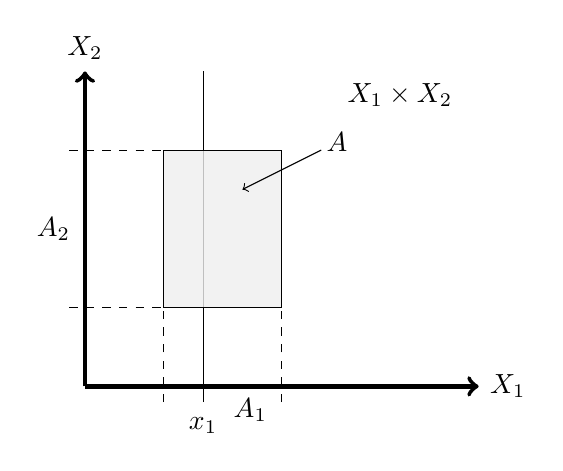
\begin{tikzpicture}
		\draw[->,ultra thick] (0,0)--(5,0) node[right]{$X_1$};
		\draw[->,ultra thick] (0,0)--(0,4) node[above]{$X_2$};
		\draw[fill=gray!10] (1,3) rectangle (2.5,1);
		\draw (1.5,-.2)--(1.5,4);
		\draw[color=gray!50] (1.5,1)--(1.5,3);
		
		\draw[dashed] (-.2,3)--(2.5,3);
		\draw[dashed] (-.2,1)--(2.5,1);
		
		\draw[dashed] (1,-.2)--(1,3);
		\draw[dashed] (2.5,-.2)--(2.5,3);
		
		\node at (1.5,-.5) {$x_1$};
		\node at (-.4,2) {$A_2$};
		\node at (2.1,-.3) {$A_1$};
		
		\draw[->] (3,3)--(2,2.5);
		\node at (3.2,3.1) {$A$};
		
		\node at (4,3.7) {$X_1 \times X_2$};
		
		\end{tikzpicture}
	\end{minipage}
	\hfill
	\begin{minipage}[t]{0.4\textwidth}
		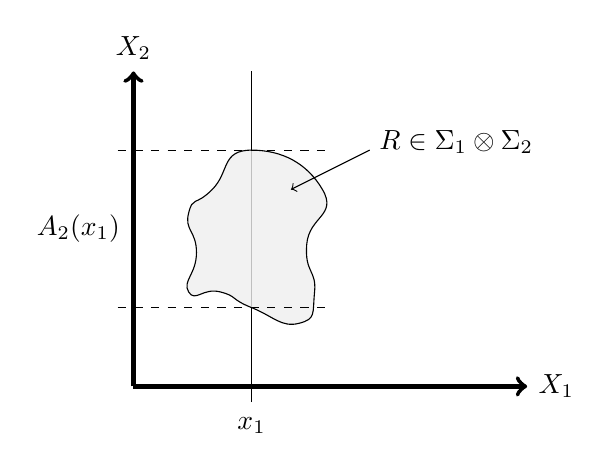
\begin{tikzpicture}
		\draw[->,ultra thick] (0,0)--(5,0) node[right]{$X_1$};
		\draw[->,ultra thick] (0,0)--(0,4) node[above]{$X_2$};
		\filldraw[fill=gray!10] plot [smooth cycle, tension = 1] coordinates {(.7,2.2) (1,2.5) (1.5,3) (2.4,2.5) (2.2,1.8) (2.3,1.2) (2.1,.8) (1.5,1) (1.1,1.2) (.7,1.2) (.8,1.7)};
		\draw (1.5,-.2)--(1.5,4);
		\draw[color=gray!50] (1.5,1)--(1.5,3);
		
		\draw[dashed] (-.2,3)--(2.5,3);
		\draw[dashed] (-.2,1)--(2.5,1);
		
		\node at (1.5,-.5) {$x_1$};
		\node at (-.7,2) {$A_2(x_1)$};
		
		\draw[->] (3,3)--(2,2.5);
		\node at (4.1,3.1) {$R \in \Sigma_1\otimes\Sigma_2$};
		\end{tikzpicture}
	\end{minipage}
	\begin{proof}
		Setze $S = \{A \in \Sigma_1\otimes\Sigma_2 \mid A_1(x_2)\in\Sigma_1\}$. Natürlich ist $A_1\times A_2 \in S$ \\
		für alle $A_1\in\Sigma_1$, $A_2\in\Sigma_2$. Insofern genügt es zu zeigen, dass $S$ eine $\sigma$-Algebra ist. \\
		In der Tat ist $X_1 \times X_2 \in S$ und für $A \in S$ ist
		\[
			\left(\cp{A}\right)_1(x_2) = \left\{x_1 \mid (x_1,x_2) \in \cp{A}\right\}
			= \cp{\{x_1 \mid (x_1,x_2) \in A\}}
			= \cp{(\underbrace{A_1(x_2)}_{\mathrlap{\in\Sigma_1}})} \in \Sigma_1.
		\]
		Für $(A_k)_{k\in\N} \subset S$ haben wir
		\[
			\left( \bigcup_{k\in\N} A_k \right)_1(x_2)
			= \left\{ x_1\ \Big\vert\ (x_1,x_2) \in \bigcup_{k\in\N}A_k \right\}
			= \bigcup_{k\in\N}\underbrace{\{x_1 \mid (x_1,x_2) \in A_k\}}_{= (A_k)_1(x_2) \in \Sigma_1} \in \Sigma_1
		\]
		Für $A_2(x_1)$ argumentiere analog.
	\end{proof}

	\begin{cor}
		Seien $(X_1,\Sigma_1)$, $(X_2,\Sigma_2)$ Messräume und sei $f \colon (X_1 \times X_2, \Sigma_1 \otimes \Sigma_2) \to (\mbb{R},\mc{B})$ messbar. \\
		Dann ist  $x_1 \mapsto f(x_1,x_2)$ für jedes $x_2 \in X_2$ auf $X_1$ messbar und entsprechend $x_2 \mapsto f(x_1,x_2)$ für jedes $x_1 \in X_1$ auf $X_2$.
	\end{cor}
	\begin{proof}
		Für $B \in \mc{B}$ und $x_2 \in X_2$ ist $f^{-1}(\cdot,x_2)(B) \overset{\text{!}}{\in} \Sigma_1$.\\
		In der Tat haben wir $A \coloneqq f^{-1}(B) \overset{f \text{ messb.}}{\in} \Sigma_1 \otimes \Sigma_2$, also ist
		\[
			f^{-1}(\cdot,x_2)(B)
			= \{x_1 \in X_1 \mid f(x_1,x_2) \in B \}
			= \{x_1 \in X_1 \mid (x_1,x_2) \in A \}
			= A_1(x_2) \in \Sigma_1
		\]
		und \emph{Lemma 57}.
	\end{proof}

	\paragraph{Ziel:} Definiere Produktmaß $\mu_1 \otimes \mu_2$ auf $\Sigma_1 \otimes \Sigma_2$ mit
	\[
		(\ast) \quad (\mu_1 \otimes \mu_2)(A_1 \times A_2) = \mu_1(A_1)\mu_2(A_2) \quad \forall A_1\in\Sigma_1,\ A_2\in\Sigma_2
	\]
	Sind $\mu_1$ und $\mu_2$ beide $\sigma$-finit, so folgt Eindeutigkeit des Produktmaßes (Existenz müssen wir noch zeigen) aus \emph{Satz 23}.
	
	\begin{theorem}
		Sind $(X_1,\Sigma_1,\mu_1)$, $(X_2,\Sigma_2,\mu_2)$ Maßräume mit $\sigma$-finiten Maßen und $A \in \Sigma_1 \otimes \Sigma_2$. \\
		Dann sind die Abbildungen $x_1 \mapsto \mu_2(A_2(x_1))$, $x_2 \mapsto \mu_1(A_1(x_2))$ auf $X_1$ bzw. $X_2$ messbar und es gilt
		\[
			\int_{X_1} \mu_2(A_2(x_1)) \md \mu_1(x_1)
			= \int_{X_2} \mu_1(A_1(x_2)) \md \mu_2(x_2).
		\]
	\end{theorem}
	\begin{proof}
		Übungsaufgabe.
	\end{proof}

	\begin{defin}
		Seien $(X_1,\Sigma_1,\mu_1)$, $(X_2,\Sigma_2,\mu_2)$ Maßräume mit $\sigma$-finiten Maßen. \\
		Für $A \in \Sigma_1 \otimes \Sigma_2$ setzen wir
		\[
			(\mu_1 \otimes \mu_2)(A) \coloneqq
			\int_{X_1} \underbrace{\mu_2(A_2(x_1))}_{\mathrlap{
				= \int_{X_2} \rchi_A(x_1,x_2) \md \mu_2(x_2)
			}} \md \mu_1(x_1)
			= \int_{X_2} \underbrace{\mu_1(A_1(x_2))}_{\mathrlap{
					= \int_{X_1} \rchi_A(x_1,x_2) \md \mu_1(x_1)
			}} \md \mu_2(x_2)
		\]
	\end{defin}
	\begin{bem*}
		$\rchi_{A_1(x_2)}(x_1) = \rchi_A(x_1,x_2)= \rchi_{A_2(x_1)}(x_2)$
	\end{bem*}

	\begin{lem}
		Das Produktmaß ist für $\sigma$-finite Maße ebenfalls ein Maß und es ist eindeutig bezüglich $(\ast)$.
	\end{lem}
	\begin{proof}
		Eindeutigkeit: siehe oben; $(\mu_1 \otimes \mu_2)(\emptyset) = 0$ ist klar und $\sigma$-Additivität folgt mit dem Satz über monotone Konvergenz:
		\begin{align*}
			\underbrace{
				(\mu_1 \otimes \mu_2)\left(\bigcupdot_{k=1}^\tau A_k\right)
			}_{\underset{\text{vgl. Bew. Satz 12}}{\xrightarrow{\tau \to\infty}}
				(\mu_1 \otimes \mu_2)\left(\bigcupdot_{k\in\N} A_k\right)
			}
			&\darrow{\text{Def.}}{=}
			\mathlarger\int_{X_1} \mu_2 \Bigg(\underbrace{
				\left(\bigcupdot_{k=1}^\tau A_k\right)_2 (x_1)
			}_{=\bigcupdot_{k=1}^\tau (A_k)_2 (x_1)}
			\Bigg) \md \mu_1(x_1) \\
			&\darrow{\text{$\sigma$-Add.}}{=}
			\mathlarger\int_{X_1}\sum_{k=1}^\tau \mu_2((A_k)_2(x_1)) \md \mu_1(x_1)
			= \sum_{k=1}^\tau (\mu_1\otimes\mu_2)(A_k)
		\end{align*}
	\end{proof}

	\begin{theorem}[Fubini]
		Seien $(X_1,\Sigma_1,\mu_1)$, $(X_2,\Sigma_2,\mu_2)$ Maßräume mit $\sigma$-finiten Maßen und \\
		$f \colon (X_1 \times X_2, \Sigma_1\otimes\Sigma_2) \to (\mbb{R},\mc{B})$ messbar.
		\begin{enumerate}[(i)]
			\item \emph{(Tonelli)} Ist $f$ nicht-negativ, so sind $\int_{X_2}f(\cdot,x_2) \md \mu_2(x_2)$ und $\int_{X_1}f(x_1,\cdot) \md \mu_1(x_1)$ als Funktion auf $X_1$ bzw. $X_2$ beide messbar und es gilt
			\begin{align*}
				\iint\limits_{X_1 \times X_2} f(x_1,x_2) \md(\mu_1\otimes\mu_2)(x_1,x_2)
				&= \int_{X_1}\left(
					\int_{X_2}f(x_1,x_2)\md\mu_2(x_2)
				\right) \md \mu_1(x_1) \\
				&= \int_{X_2}\left(
				\int_{X_1}f(x_1,x_2)\md\mu_1(x_1)
				\right) \md \mu_2(x_2).
			\end{align*}
			
			\item Allgemein ist $f \in \mathscr{L}^1(X_1 \times X_2, \mu_1\otimes\mu_2)$ äquivalent zu
			\begin{align*}
				&\int_{X_1} |f(x_1,\cdot)| \md \mu_1(x_1) \in \mathscr{L}(X_2,\mu_2) \\
				\text{bzw.\quad} &\int_{X_2} |f(\cdot,x_2)| \md \mu_2(x_2) \in \mathscr{L}(X_1,\mu_1)
			\end{align*}
			und in diesem Fall gilt (i).
		\end{enumerate}
	\end{theorem}
	\begin{proof}
		Aufgrund der Linearität erhalten wir aus \emph{Satz 59} für  eine einfache Funktion \\
		$f = \sum_{j=1}^k \alpha_j\rchi_{A_j}$,\quad $\alpha_j \geq 0$,\quad $A_j \in \Sigma_1 \otimes \Sigma_2$,\quad $A_i \cap A_j = \emptyset$,\quad $X = \bigcup_{j=1}^k A_j$
		\[
			\int_{X_2} f(\cdot,x_2) \md \mu_2(x_2) 
			= \sum_{j=1}^k \alpha_j \underbrace{\mu_2((A_j)_2(\cdot))}_{
				\mathclap{\text{messbar nach \emph{Satz 59}}}
			}
		\]
		Weiterhin ist
		\begin{align*}
			\iint\limits_{X_1 \times X_2} f(x_1,x_2) \md(\mu_1\otimes\mu_2)(x_1,x_2)
			=& \sum_{j=1}^k \alpha_j \iint\limits_{X_1 \times X_2} \rchi_{A_j}(x_1,x_2) \md(\mu_1\otimes\mu_2)(x_1,x_2) \\
			\darrow{\text{Def. 60}}{=}& \sum_{j=1}^k 
			\alpha_j \int_{X_1} \left(\int_{X_2} \rchi_{A_j}(x_1,x_2) \md\mu_2(x_2) \right)\md\mu_1(x_1) \\
			=& \int_{X_1} \left(\int_{X_2} f(x_1,x_2) \md\mu_2(x_2) \right)\md\mu_1(x_1) \\
			= \dotsb =&  \int_{X_2} \left(\int_{X_1} f(x_1,x_2) \md\mu_1(x_1) \right)\md\mu_2(x_2)
		\end{align*}
		Sei nun $(f_k)_{k\in\N} \subset S(X_1 \times X_2,m \mu_1 \otimes \mu_2)$ mit $0 \leq f_k \nearrow f$. Dann haben wir
		\[
			\int_{X_2} f_k(\cdot,x_2) \md\mu_2(x_2) \leq \int_{X_2} f(\cdot,x_2) \md\mu_2(x_2) \quad \forall k \in \N
		\]
		und
		\[
			\lim_{k\to\infty} \int_{X_2} f_k(\cdot,x_2) \md\mu_2(x_2) \darrow{\text{Satz 45}}{=} \int_{X_2} f(\cdot,x_2) \md\mu_2(x_2)
		\]
		Nun sind erneut die Voraussetzungen für \emph{Satz 45} erfüllt und wir erhalten
		\begin{align*}
			\lim_{k \to \infty} \int_{X_1} \int_{X_2} f_k(x_1,x_2) \md\mu_2(x_2) \md\mu_1(x_1)
			&= \int_{X_1} \lim_{k \to \infty} \int_{X_2} f_k(x_1,x_2) \md\mu_2(x_2) \md\mu_1(x_1) \\
			&= \int_{X_1} \int_{X_2} f(x_1,x_2) \md\mu_2(x_2) \md\mu_1(x_1)
		\end{align*}
		Genauso mit 1 und 2 vertauscht.\\
		Einmalige Anwendung von \emph{Satz 45} liefert
		\[
			\lim_{k\to\infty} \iint\limits_{X_1 \times X_2} f_k(x_1,x_2) \md(\mu_1\otimes\mu_2)(x_1,x_2)
			= \iint\limits_{X_1 \times X_2} f(x_1,x_2) \md(\mu_1\otimes\mu_2)(x_1,x_2)
		\]
		\emph{(ii)} folgt sofort auf \emph{(i)} mit $f=f^+ - f^-$ und $|f| = f^+ + f^-$.
		\paragraph{Erinnerung: } $f\in\mathscr{L}^1(X_1 \times X_2) \iff \iint |f| \md(\mu_1\otimes\mu_2)(x_1,x_2) < \infty$.
	\end{proof}
	
\end{document}